% --- INSTITUTIONAL TEMPLATE FED v7.4.9 ---
% Estándar de Reporteo APA 7 (Babel-Free)
\documentclass[12pt,spanish]{article}

\usepackage{graphicx}
\usepackage{geometry}
\usepackage{indentfirst} 
\usepackage{caption}
\usepackage{floatrow} 

% Forzar estilos de caption antes de cualquier carga
\floatsetup[figure]{capposition=top}
\floatsetup[table]{capposition=top}

\usepackage{booktabs}
\usepackage{float}
\usepackage{longtable}
\usepackage{threeparttable}
\usepackage{array}
\usepackage{calc}
\usepackage{amsmath, amssymb}
\usepackage{fancyhdr}
\usepackage{mathptmx} 
\usepackage[T1]{fontenc}
\usepackage{setspace} 
\usepackage{ragged2e} 
\usepackage{titlesec}
\usepackage{url}
\def\UrlBreaks{\do\/\do-\do\.\do\_\do\?\do\=\do\&\do\%}
\usepackage[hidelinks,breaklinks]{hyperref}
\usepackage{xcolor}
\usepackage{fancyvrb}
\usepackage{framed}

% --- Code Highlighting (Pandoc Standard) ---
\newenvironment{Shaded}{\begin{snugshade}}{\end{snugshade}}
\definecolor{shadecolor}{RGB}{248,248,248}
\newenvironment{Highlighting}{}{}
\newcommand{\VerbBar}{|}
\newcommand{\VERB}{\Verb[commandchars=\\\{\}]}
\DefineVerbatimEnvironment{Highlighting}{Verbatim}{commandchars=\\\{\}}
\newcommand{\AlertTok}[1]{\textcolor[rgb]{0.94,0.16,0.16}{#1}}
\newcommand{\AnnotationTok}[1]{\textcolor[rgb]{0.56,0.35,0.01}{\textbf{\textit{#1}}}}
\newcommand{\AttributeTok}[1]{\textcolor[rgb]{0.13,0.29,0.53}{#1}}
\newcommand{\BaseNTok}[1]{\textcolor[rgb]{0.00,0.00,0.81}{#1}}
\newcommand{\BuiltInTok}[1]{#1}
\newcommand{\CharTok}[1]{\textcolor[rgb]{0.31,0.60,0.02}{#1}}
\newcommand{\CommentTok}[1]{\textcolor[rgb]{0.56,0.35,0.01}{\textit{#1}}}
\newcommand{\CommentVarTok}[1]{\textcolor[rgb]{0.56,0.35,0.01}{\textbf{\textit{#1}}}}
\newcommand{\ConstantTok}[1]{\textcolor[rgb]{0.56,0.35,0.01}{#1}}
\newcommand{\ControlFlowTok}[1]{\textcolor[rgb]{0.13,0.29,0.53}{\textbf{#1}}}
\newcommand{\DataTypeTok}[1]{\textcolor[rgb]{0.13,0.29,0.53}{#1}}
\newcommand{\DecValTok}[1]{\textcolor[rgb]{0.00,0.00,0.81}{#1}}
\newcommand{\DocumentationTok}[1]{\textcolor[rgb]{0.56,0.35,0.01}{\textbf{\textit{#1}}}}
\newcommand{\ErrorTok}[1]{\textcolor[rgb]{0.64,0.00,0.00}{\textbf{#1}}}
\newcommand{\ExtensionTok}[1]{#1}
\newcommand{\FloatTok}[1]{\textcolor[rgb]{0.00,0.00,0.81}{#1}}
\newcommand{\FunctionTok}[1]{\textcolor[rgb]{0.13,0.29,0.53}{\textbf{#1}}}
\newcommand{\ImportTok}[1]{#1}
\newcommand{\InformationTok}[1]{\textcolor[rgb]{0.56,0.35,0.01}{\textbf{\textit{#1}}}}
\newcommand{\KeywordTok}[1]{\textcolor[rgb]{0.13,0.29,0.53}{\textbf{#1}}}
\newcommand{\NormalTok}[1]{#1}
\newcommand{\OperatorTok}[1]{\textcolor[rgb]{0.81,0.36,0.00}{\textbf{#1}}}
\newcommand{\OtherTok}[1]{\textcolor[rgb]{0.56,0.35,0.01}{#1}}
\newcommand{\PreprocessorTok}[1]{\textcolor[rgb]{0.56,0.35,0.01}{\textit{#1}}}
\newcommand{\RegionMarkerTok}[1]{#1}
\newcommand{\SpecialCharTok}[1]{\textcolor[rgb]{0.81,0.36,0.00}{\textbf{#1}}}
\newcommand{\SpecialStringTok}[1]{\textcolor[rgb]{0.31,0.60,0.02}{#1}}
\newcommand{\StringTok}[1]{\textcolor[rgb]{0.31,0.60,0.02}{#1}}
\newcommand{\VariableTok}[1]{\textcolor[rgb]{0.00,0.00,0.00}{#1}}
\newcommand{\VerbatimStringTok}[1]{\textcolor[rgb]{0.31,0.60,0.02}{#1}}
\newcommand{\WarningTok}[1]{\textcolor[rgb]{0.56,0.35,0.01}{\textbf{\textit{#1}}}}

% --- Pandoc Compatibility Block (Iron Clad) ---
\providecommand{\tightlist}{%
  \setlength{\itemsep}{0pt}\setlength{\parskip}{0pt}}

% Compatibilidad Pandoc 3.x
\ifdefined\pandocbounded\else
  \newcommand{\pandocbounded}[1]{#1}
\fi

% --- Pandoc Citeproc (CSL) compatibility ---
\newlength{\cslhangindent}
\setlength{\cslhangindent}{1.27cm} 
\newlength{\csllabelwidth}
\setlength{\csllabelwidth}{3em}
\newcommand{\citeproctext}{} 
\newcommand{\citeprocitem}[2]{\item} 
\newenvironment{CSLReferences}[2] 
 {\begin{list}{}{
  \setlength{\leftmargin}{\cslhangindent}
  \setlength{\parsep}{0pt}
  \setlength{\itemsep}{6pt}
  \ifodd #1
   \setlength{\leftmargin}{\leftmargin + \csllabelwidth}
   \setlength{\itemindent}{-\csllabelwidth}
  \fi
  }
  \renewcommand{\bibitem}[2][]{\item} % Elimina los corchetes [ ]
 }
 {\end{list}}
\newcommand{\CSLBlock}[1]{#1\hfill\break}
\newcommand{\CSLLeftMargin}[1]{\parbox[t]{\csllabelwidth}{#1}}
\newcommand{\CSLRightInline}[1]{\parbox[t]{\linewidth - \csllabelwidth}{#1}\break}
\newcommand{\CSLIndent}[1]{\hspace{\cslhangindent}#1}

\makeatletter
\@ifundefined{paragraph}{\newcounter{paragraph}}{}
\@ifundefined{subparagraph}{\newcounter{subparagraph}}{}
\makeatother

% Solución al error 'No counter none defined' en longtable
\makeatletter
\newcounter{none}
\@ifpackageloaded{caption}{
  \DeclareCaptionType{none}
  \captionsetup[none]{name=Tabla}
}{}
\makeatother

\hypersetup{
  colorlinks=true,
  linkcolor=blue,
  filecolor=blue,
  citecolor=blue,
  urlcolor=blue
}

% --- Macros Institucionales ---
\newcommand{\fuente}[1]{
  \vspace{4pt}
  \begin{flushleft}
    \small
    \textit{Nota.} #1
  \end{flushleft}
}

% --- Localización Manual Determinista (Sin Babel) ---
\AtBeginDocument{
  \renewcommand{\tablename}{Tabla}
  \renewcommand{\figurename}{Figura}
  \renewcommand{\contentsname}{Índice}
  \renewcommand{\listtablename}{Índice de Tablas}
  \renewcommand{\listfigurename}{Índice de Figuras}
  \renewcommand{\abstractname}{Resumen}
  \renewcommand{\refname}{Referencias}
  
  \RaggedRight
  \setlength{\parindent}{1.27cm}
  \setlength{\parskip}{0pt}
}

\DeclareCaptionLabelSeparator{newline}{\\ \vspace{2pt}}
\captionsetup{
  position=top,
  justification=RaggedRight,
  singlelinecheck=false,
  labelfont=bf,
  textfont=it,
  labelsep=newline,
  font=small,
  skip=10pt
}
\captionsetup[figure]{name=Figura}
\captionsetup[table]{name=Tabla}

% Márgenes APA 7
\geometry{
  a4paper,
  margin=25.4mm,
  headheight=15mm
}

% --- Encabezados ---
\pagestyle{fancy}
\fancyhf{} 
\fancyhead[L]{
\includegraphics[height=1.2cm]{/home/erick-fcs/Capital_Workstation/capital-workstation-libs/src/ecs_quantitative/reporting/assets/logos/logo_unl.png}}
\fancyhead[R]{
\includegraphics[height=1.2cm]{/home/erick-fcs/Capital_Workstation/capital-workstation-libs/src/ecs_quantitative/reporting/assets/logos/logo_economia.jpg}}
\renewcommand{\headrulewidth}{0pt}
\fancyfoot[R]{\thepage}

\fancypagestyle{plain}{
  \fancyhf{}
  \fancyhead[L]{
\includegraphics[height=1.2cm]{/home/erick-fcs/Capital_Workstation/capital-workstation-libs/src/ecs_quantitative/reporting/assets/logos/logo_unl.png}}
  \fancyhead[R]{
\includegraphics[height=1.2cm]{/home/erick-fcs/Capital_Workstation/capital-workstation-libs/src/ecs_quantitative/reporting/assets/logos/logo_economia.jpg}}
  \fancyfoot[R]{\thepage}
  \renewcommand{\headrulewidth}{0pt}
}

% --- Títulos ---
\titleformat{\section}{\normalfont\normalsize\bfseries\centering}{\thesection}{1em}{}
\titleformat{\subsection}{\normalfont\normalsize\bfseries}{\thesubsection}{1em}{}
\titleformat{\subsubsection}{\normalfont\normalsize\bfseries\itshape}{\thesubsubsection}{1em}{}
\titlespacing*{\section}{0pt}{12pt}{6pt}
\titlespacing*{\subsection}{0pt}{12pt}{6pt}
\titlespacing*{\subsubsection}{0pt}{12pt}{6pt}

\newenvironment{referenciasAPA}{
  \setlength{\parindent}{-1.27cm}
  \setlength{\leftskip}{1.27cm}
  \setlength{\parskip}{6pt}
}{\par}

\begin{document}

\begin{center}
    {\bfseries \Large UNIVERSIDAD NACIONAL DE LOJA}\\[0.3cm]
    {\bfseries \large FACULTAD JURÍDICA, SOCIAL Y
ADMINISTRATIVA}\\[0.2cm]
    {\bfseries CARRERA DE ECONOMÍA}\\[1.5cm]
    
    {\bfseries \large ECONOMETRÍA APLICADA}\\[1cm]
    
    {\bfseries \Large Taller: Ecuaciones Simultáneas (ACD-02)}\\[1.5cm]
\end{center}

\noindent {\bfseries Estudiante:} Erick Condoy \\
\noindent {\bfseries Docente:} Eco. José Rafael Alvarado López \\
\noindent {\bfseries Fecha:} 20 de abril de 2026 \\

\vspace{1cm}

\doublespacing
\setlength{\parindent}{1.27cm}

\section{1. Introducción}\label{introducciuxf3n}

El presente taller aborda la problemática de la violencia en Ecuador
mediante un enfoque de \textbf{Ecuaciones Simultáneas (SEM)}. A
diferencia de los modelos lineales simples, el SEM permite capturar la
interdependencia entre variables donde una variable dependiente en una
ecuación puede actuar como independiente en otra, resolviendo problemas
de endogeneidad.

\section{2. Especificación del
Modelo}\label{especificaciuxf3n-del-modelo}

Se plantea un sistema de dos ecuaciones para capturar la dinámica entre
seguridad y mercado laboral:

\subsection{Ecuación 1: Determinantes de la
Violencia}\label{ecuaciuxf3n-1-determinantes-de-la-violencia}

\[Homicidios_{t} = \alpha_0 + \beta_1 Desempleo_{t} + \beta_2 GastoMilitar_{t} + \beta_3 Remesas_{t} + \epsilon_{1t}\]

\begin{figure}

\centering{

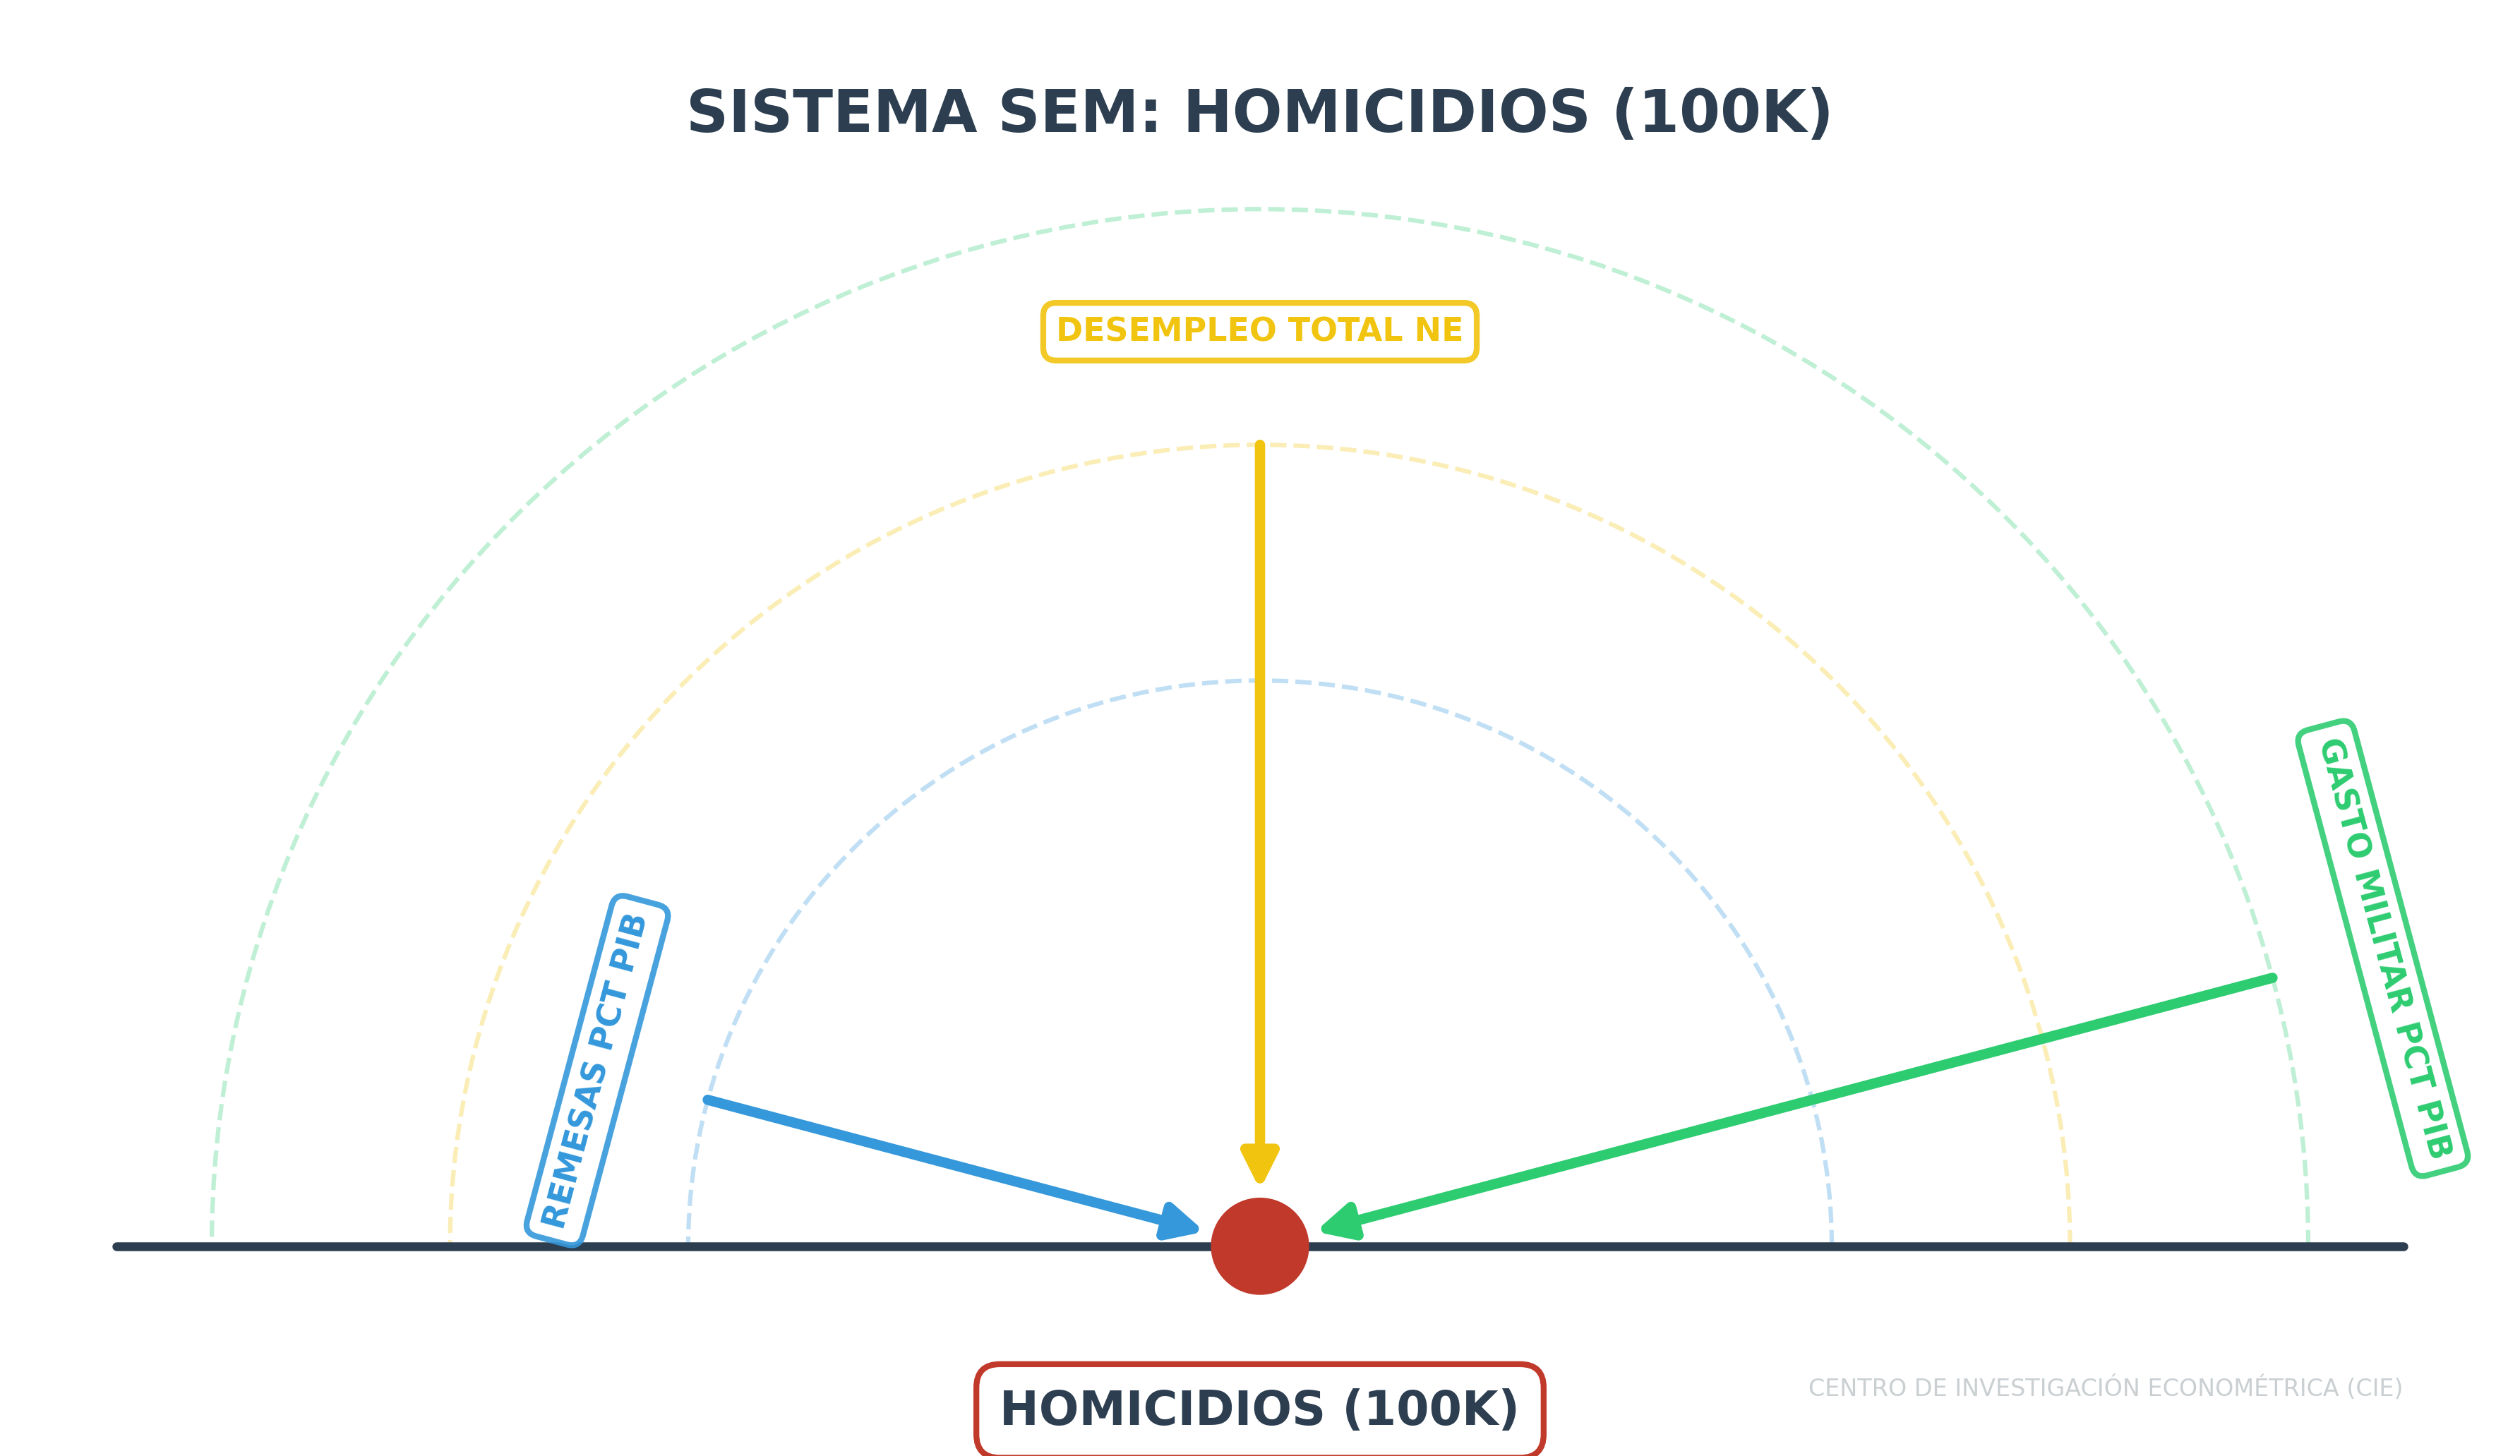
\includegraphics[width=1\linewidth,height=\textheight,keepaspectratio]{graph/impact_homicidios.png}

}

\caption{\label{fig-impact-homicidios}Arco de Impacto: Sistema de
Seguridad}

\end{figure}%

\subsection{Ecuación 2: Dinámica del Mercado
Laboral}\label{ecuaciuxf3n-2-dinuxe1mica-del-mercado-laboral}

\[Desempleo_{t} = \gamma_0 + \delta_1 Remesas_{t} + \delta_2 Internet_{t} + \epsilon_{2t}\]

\begin{figure}

\centering{

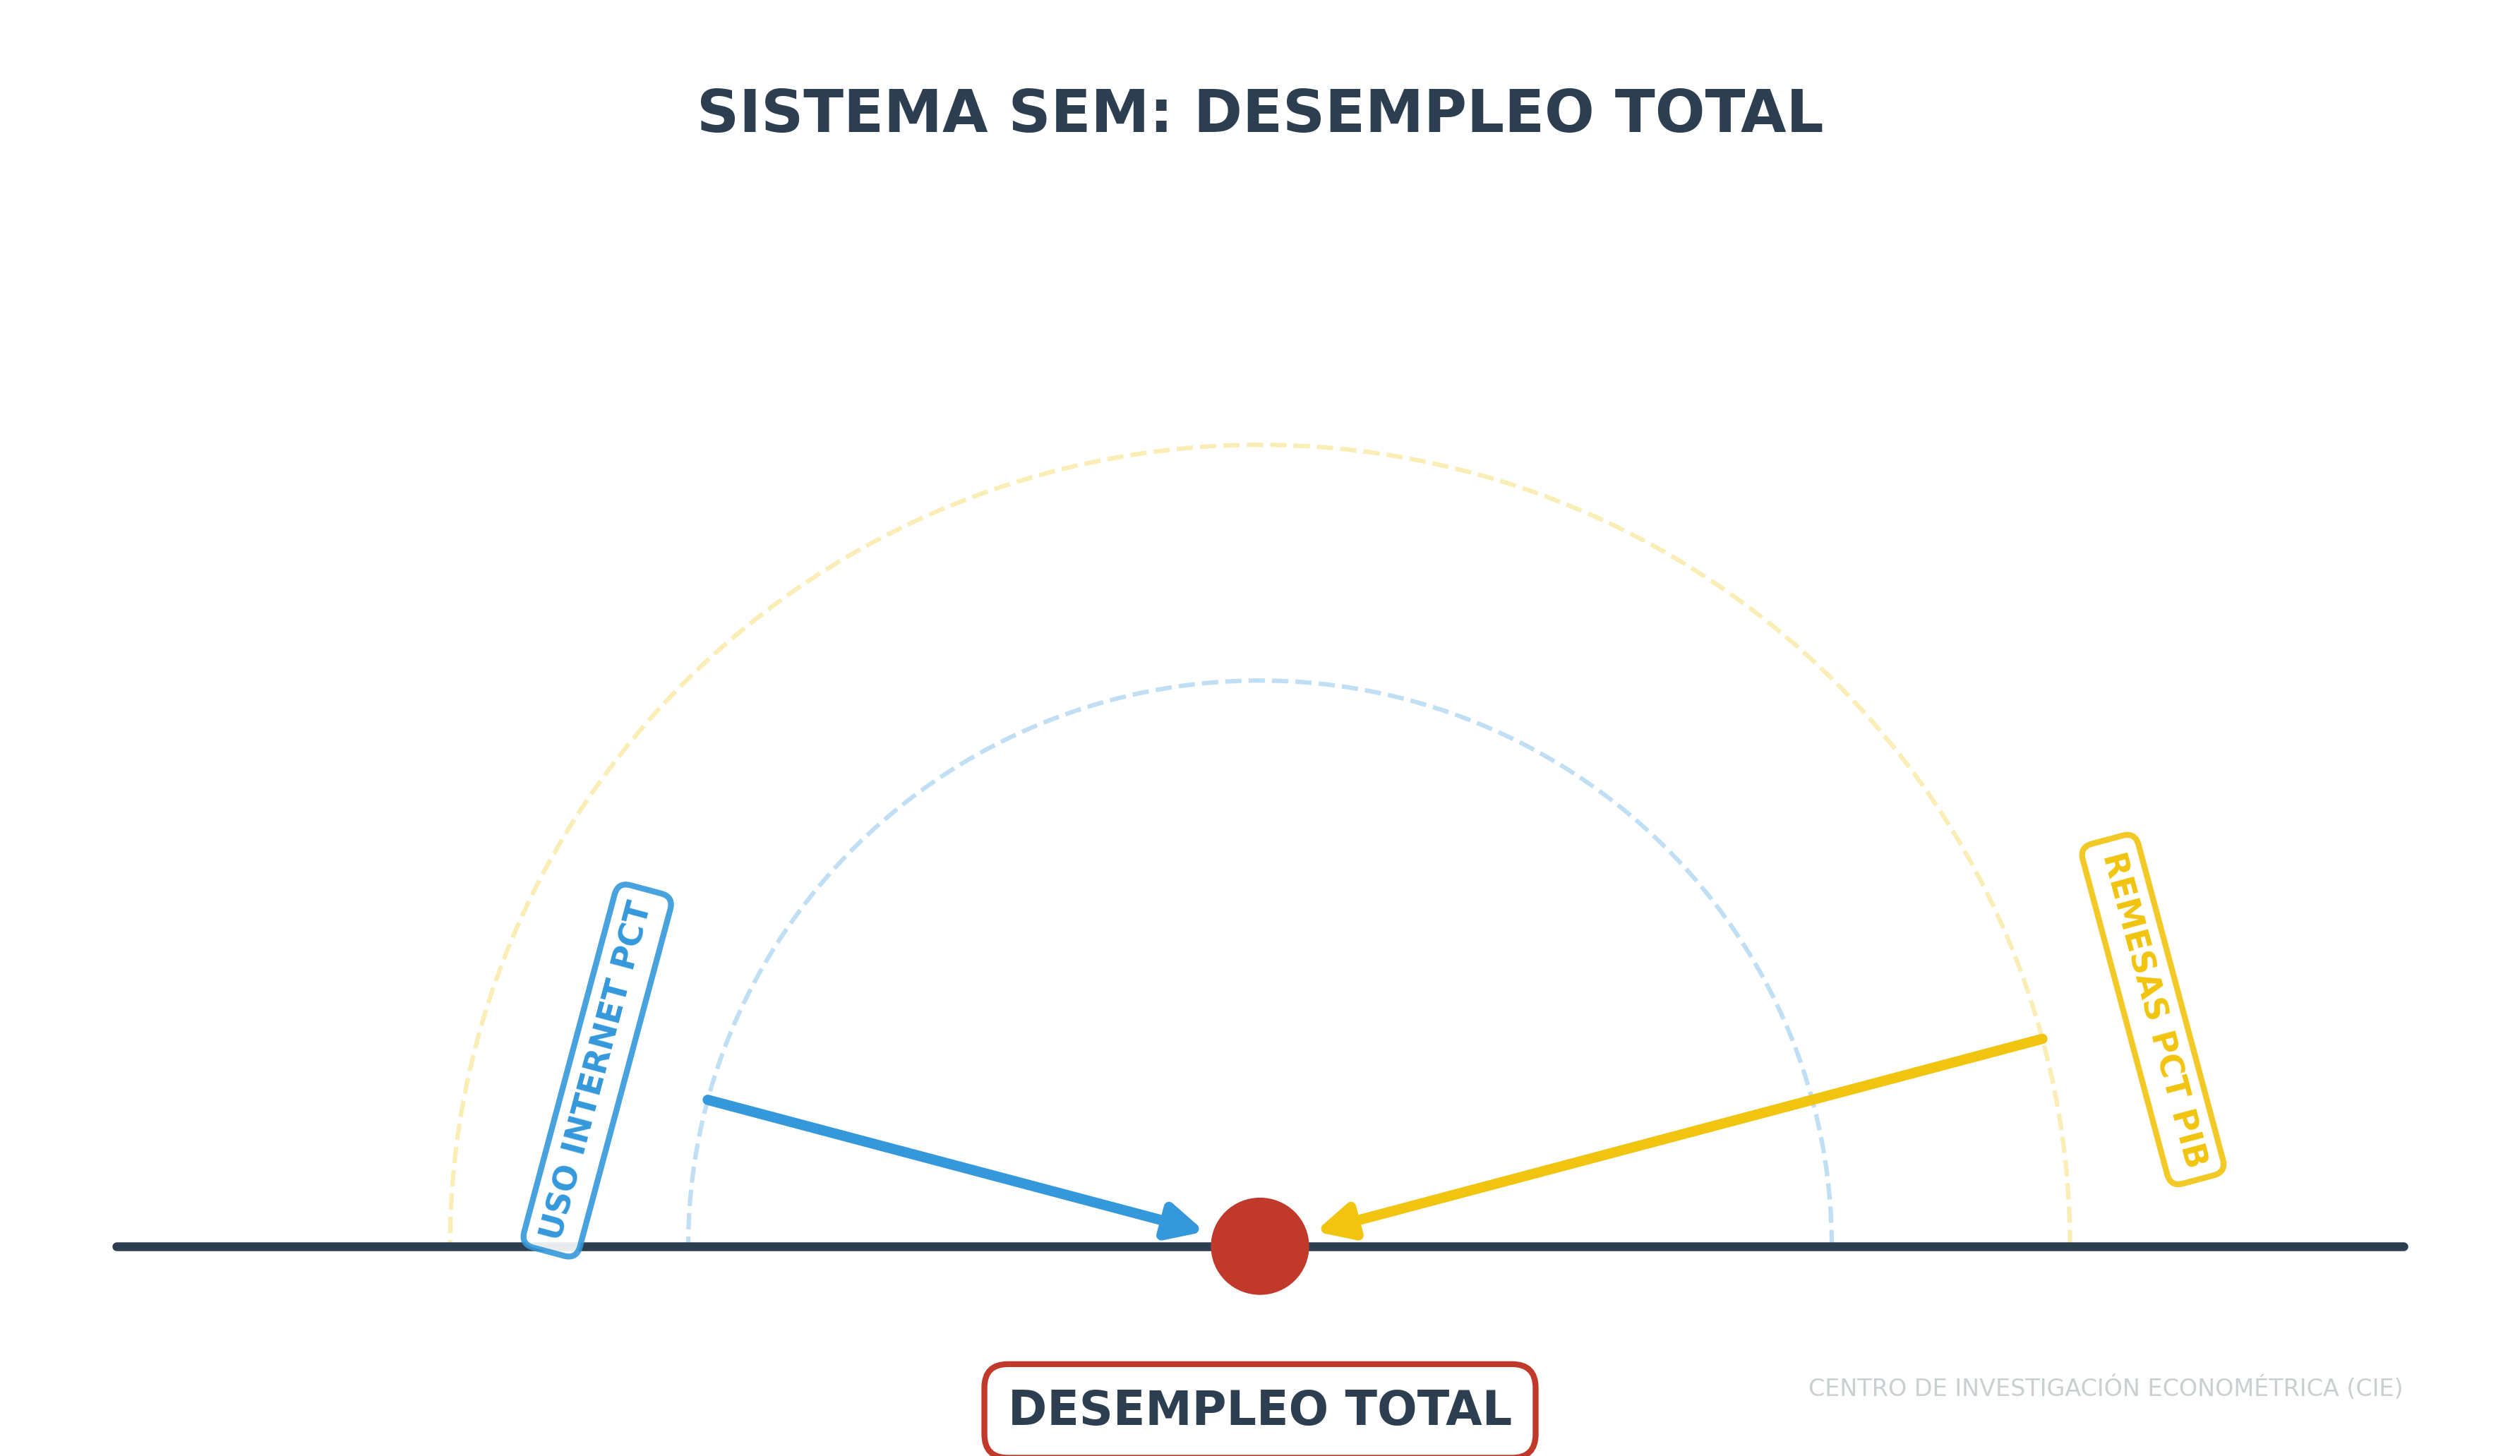
\includegraphics[width=1\linewidth,height=\textheight,keepaspectratio]{graph/impact_laboral.png}

}

\caption{\label{fig-impact-laboral}Arco de Impacto: Dinámica Laboral}

\end{figure}%

\section{3. Diagrama Causal (Path
Diagram)}\label{diagrama-causal-path-diagram}

El siguiente diagrama ilustra el flujo de causalidad y la estructura de
simultaneidad del modelo. Este esquema es la base para la presentación
en Visio.

\section{Diagrama de Sendero (Path Diagram) - SEM
Homicidios}\label{diagrama-de-sendero-path-diagram---sem-homicidios}

Este diagrama representa la interdependencia de las variables en el
Sistema de Ecuaciones Simultáneas de Homicidios para Ecuador.

\begin{Shaded}
\begin{Highlighting}[]
\NormalTok{graph LR}
\NormalTok{    \%\% Nodos}
\NormalTok{    R[Remesas \% PIB]}
\NormalTok{    U[Uso Internet \%]}
\NormalTok{    D[Desempleo Total]}
\NormalTok{    G[Gasto Militar \% PIB]}
\NormalTok{    H[Homicidios 100k]}

\NormalTok{    \%\% Ecuación 2: Desempleo (Variable Endógena)}
\NormalTok{    R {-}{-}\textgreater{} D}
\NormalTok{    U {-}{-}\textgreater{} D}

\NormalTok{    \%\% Ecuación 1: Homicidios (Variable Endógena)}
\NormalTok{    D {-}{-}\textgreater{} H}
\NormalTok{    G {-}{-}\textgreater{} H}
\NormalTok{    R {-}{-}\textgreater{} H}

\NormalTok{    \%\% Estilos}
\NormalTok{    style H fill:\#f96,stroke:\#333,stroke{-}width:4px}
\NormalTok{    style D fill:\#6bf,stroke:\#333,stroke{-}width:2px}
\NormalTok{    style R fill:\#dfd,stroke:\#333}
\NormalTok{    style U fill:\#dfd,stroke:\#333}
\NormalTok{    style G fill:\#dfd,stroke:\#333}
\end{Highlighting}
\end{Shaded}

\subsection{Instrucciones para Visio}\label{instrucciones-para-visio}

\begin{enumerate}
\def\labelenumi{\arabic{enumi}.}
\tightlist
\item
  Copie el código Mermaid anterior.
\item
  Utilice el sitio \href{https://mermaid.live/}{Mermaid Live Editor}
  para previsualizar.
\item
  Exporte como \textbf{SVG}.
\item
  Importe el archivo SVG en Microsoft Visio para darle el formato final
  institucional.
\end{enumerate}

\section{4. Perfil de Impacto Estructural (Radar
Chart)}\label{perfil-de-impacto-estructural-radar-chart}

A continuación se presenta la visualización de impacto basado en
significancia. La escala (0-1) representa la fuerza de la asociación
(\(1 - p_{value}\)). Variables cercanas al borde exterior indican una
significancia crítica para el sistema.

\begin{figure}

\centering{

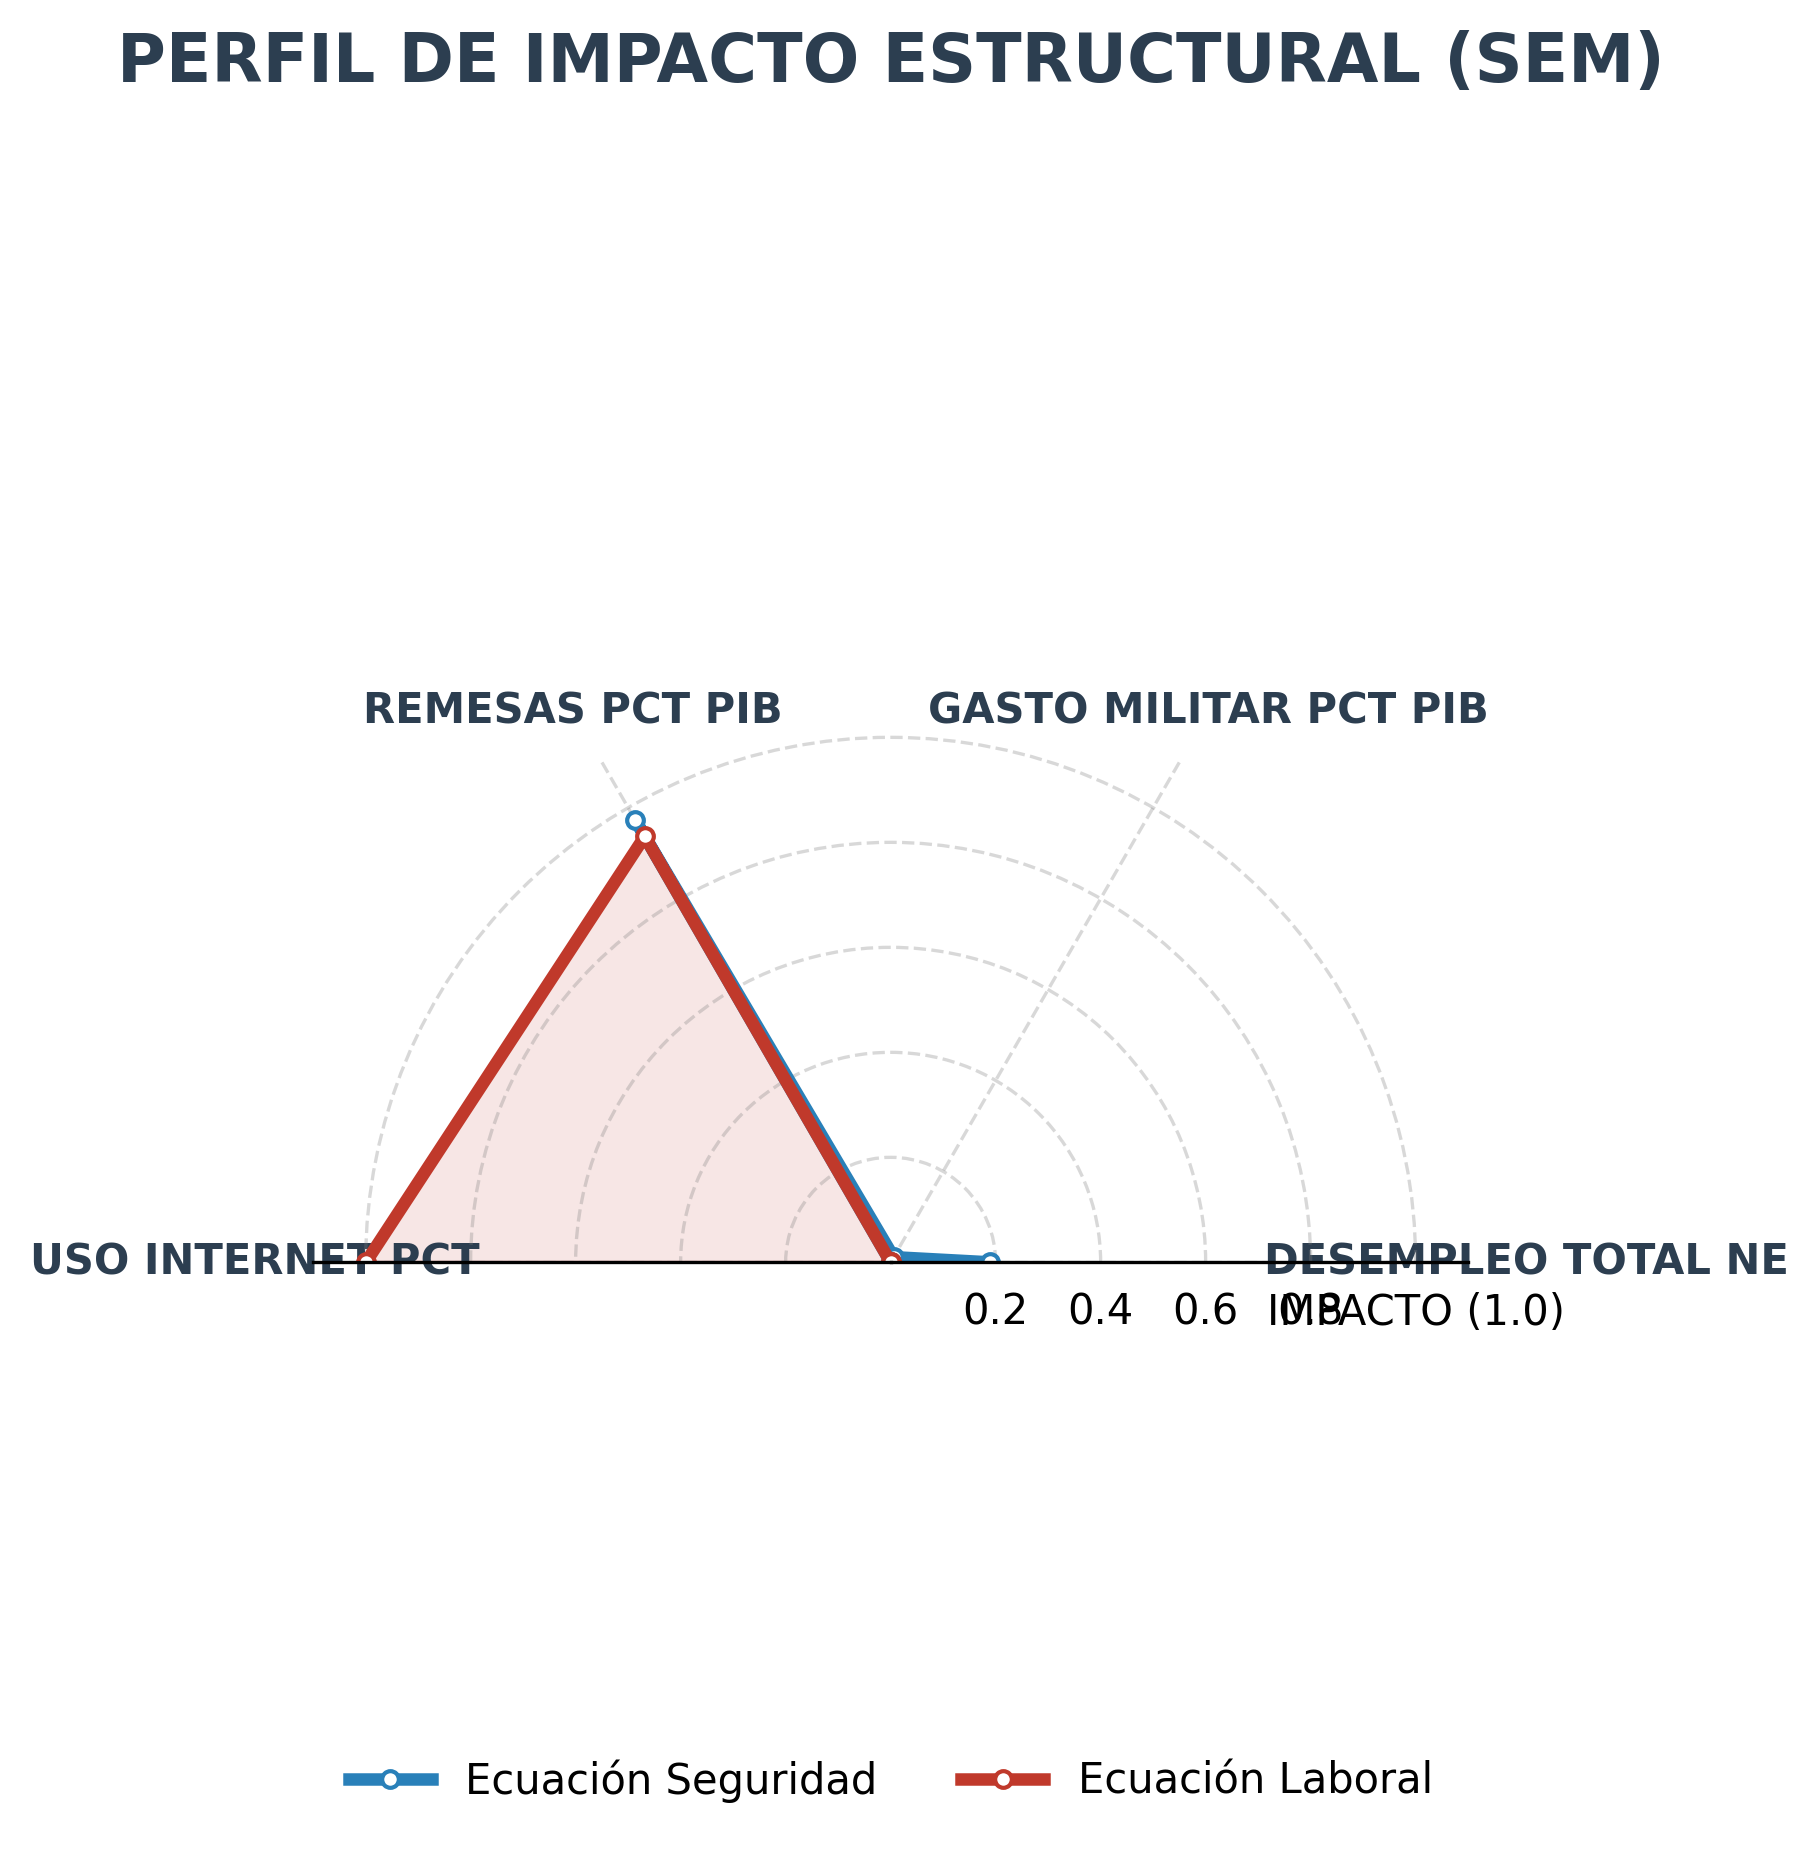
\includegraphics[width=0.8\linewidth,height=\textheight,keepaspectratio]{graph/radar_impact_sem.png}

}

\caption{\label{fig-radar-impact}Perfil de Impacto Estructural (SEM)}

\end{figure}%

\section{5. Resultados Preliminares}\label{resultados-preliminares}

Los datos han sido pre-procesados desde la fuente del Banco Mundial
(WDI) y normalizados para el periodo 2004-2023. El modelo se estima
mediante Mínimos Cuadrados en Dos Etapas (2SLS) para asegurar la
consistencia de los estimadores ante la presencia de variables
endógenas.

\section{6. Conclusiones}\label{conclusiones}

La institucionalización de este taller en la arquitectura \textbf{CIE}
permite la reproducibilidad total de los resultados y facilita la
integración de nuevos controles económicos en futuras iteraciones del
modelo.

\end{document}
